%(BEGIN_QUESTION)
% Copyright 2007, Tony R. Kuphaldt, released under the Creative Commons Attribution License (v 1.0)
% This means you may do almost anything with this work of mine, so long as you give me proper credit

Her vises skjemaet for en full ``PID'' analog elektronisk regulator. Selv om den mangler funksjonene utgangs- og setpunktsporing, har den alle tre reguleringsledd: proporsjonal, integral og derivat.

$$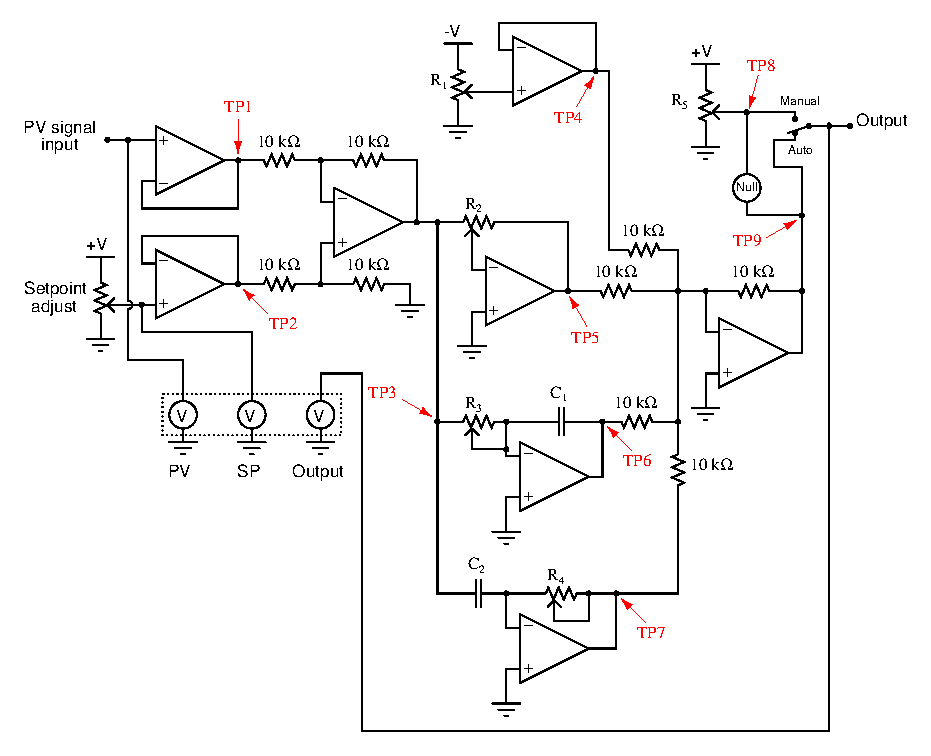
\includegraphics[width=15.5cm]{i01635x01.eps}$$

Basert på analysen din av denne kretsen, svar på følgende spørsmål:

\begin{itemize}
\item{}Ved hvilket testpunkt ville du målt regulatorens derivatledd-signal?
\vskip 5pt
\item{}Ved hvilket testpunkt ville du målt regulatorens avvikssignal?
\vskip 5pt
\item{}Ved hvilket testpunkt ville du målt regulatorens setpunktsignal?
\vskip 5pt
\item{}Hvilket potensiometer justerer integralkonstanten ($\tau_i$)?
\vskip 5pt
\item{}Hvilket potensiometer justerer derivatkonstanten ($\tau_d$)?
\vskip 5pt
\item{}Hvilken kondensator brukes til å beregne integralleddet?
\vskip 5pt
\item{}Vil justering av proporsjonalkonstanten påvirke enten integral- eller derivatresponsen?
\end{itemize} 

\vfil 

\underbar{file i01635}
\eject
%(END_QUESTION)





%(BEGIN_ANSWER)

Dette er et vurdert spørsmål -- ingen svar eller hint er gitt!

%(END_ANSWER)





%(BEGIN_NOTES)

For å svare på disse spørsmålene må du først identifisere funksjonen til hver krets-``modul'' i regulatoren korrekt.

\vskip 10pt

{\it Ved hvilket testpunkt ville du målt regulatorens derivatledd-signal?}

Ved {\bf TP7}, rett på utgangen av nederste operasjonsforsterker der derivatleddet beregnes.
 
\vskip 10pt

{\it Ved hvilket testpunkt ville du målt regulatorens avvikssignal?}

På utgangen av differensialforsterkeren, ved {\bf TP3}.
 
\vskip 10pt

{\it Ved hvilket testpunkt ville du målt regulatorens setpunktsignal?}

På utgangen av bufferen til setpunktpotensiometeret, {\bf TP2}.
 
\vskip 10pt

{\it Hvilket potensiometer justerer integralkonstanten ($\tau_i$)?}

Potensiometer {\bf R3} ved inngangen til operasjonsforsterkeren.
 
\vskip 10pt

{\it Hvilket potensiometer justerer derivatkonstanten ($\tau_d$)?}

Potensiometer {\bf R4} i tilbakekoblingssløyfen til operasjonsforsterkeren.
 
\vskip 10pt

{\it Hvilken kondensator brukes til å beregne integralleddet?}

Kondensator {\bf C1}, som står i serie med potensiometer $R_3$.
 
\vskip 10pt

{\it Vil justering av proporsjonalkonstanten påvirke enten integral- eller derivatresponsen?}

Nei, fordi utgangen fra den inverterende forsterkeren (der potensiometer $R_2$ setter forsterkningen) ikke er koblet til inngangene til hverken integral- eller derivatdelen av regulatoren. Utgangen fra proporsjonaldelen summeres bare med signalene fra integral- og derivatledd (samt bias-signalet). Dette gjør at P-, I- og D-konstantene er uavhengige av hverandre.
 
%INDEX% Control, proportional + integral + derivative: analog electronic controller

%(END_NOTES)
